\chapter{拉格朗日动力学}
\label{ch:3}

\section*{3.1  达朗贝尔原理}

乘以 $\delta r_\alpha$ 不会产生任何影响。此外，对所有质点求和只不过是把若干全为零的项相加。因此，这个表达式等于零这一事实显然是正确的。目前还不太明显的是，为什么这种特殊的表述会有什么价值。

我们从用笛卡尔坐标表示达朗贝尔原理入手，然后变换到广义坐标。对于 $N$ 个质点，有 $n = 3N$ 个笛卡尔坐标，我们可以把达朗贝尔原理写成如下的标量形式：
\[
\sum_{i=1}^{n}\left(F_i^{\mathrm{ext}} - \dot{p}_i\right)\delta\xi_i = 0.
\tag{3.3}
\]
如果有 $n$ 个笛卡尔坐标和 $k$ 个约束，我们（原则上）可以用 $n - k$ 个广义坐标来表述这个问题。变换方程为
\[
\begin{aligned}
x_1 &= x_1(q_1, q_2, \ldots, q_{n-k}, t),\\
x_2 &= x_2(q_1, q_2, \ldots, q_{n-k}, t),\\
&\vdots\\
x_n &= x_n(q_1, q_2, \ldots, q_{n-k}, t).
\end{aligned}
\]
注意，尽管有 $n$ 个笛卡尔坐标 $\xi_i$，却只有 $n - k$ 个广义坐标，因为每个约束都会使自由度数减少一个，从而也减少广义坐标的数目。

式(3.2)中的量 $\delta r_i$ 或式(3.3)中的 $\delta\xi_i$ 是虚位移。根据方程(1.9)，
\[
\delta\xi_i = \sum_{j=1}^{n-k}\frac{\partial\xi_i}{\partial q_j}\delta q_j.
\]
因此，达朗贝尔原理中的第一项可以写成
\[
\sum_i F_i^{\mathrm{ext}}\delta\xi_i = \sum_i F_i^{\mathrm{ext}}\left(\sum_j\frac{\partial\xi_i}{\partial q_j}\delta q_j\right) = \sum_{i,j}F_i^{\mathrm{ext}}\frac{\partial\xi_i}{\partial q_j}\delta q_j = \sum_j Q_j\delta q_j.
\]
最后一个量就是"虚功"。（它是在虚位移过程中所做的功。参见第 1.6 节。）

接下来考虑达朗贝尔原理中的另一项，即 $\dot{p}_i\delta\xi_i$：
\[
\sum_i\dot{p}_i\delta\xi_i = \sum_i\dot{p}_i\sum_j\frac{\partial\xi_i}{\partial q_j}\delta q_j = \sum_i m_i\ddot{x}_i\sum_j\frac{\partial\xi_i}{\partial q_j}\delta q_j,
\]
其中我们假定质点的质量恒定不变。但是，
\[
\frac{d}{dt}\left(m_i\dot{x}_i\frac{\partial\xi_i}{\partial q_j}\right) = m_i\ddot{x}_i\frac{\partial\xi_i}{\partial q_j} + m_i\dot{x}_i\frac{d}{dt}\left(\frac{\partial\xi_i}{\partial q_j}\right).
\]
回想方程(1.7)：
\[
\frac{\partial\xi_i}{\partial q_j} = \frac{\partial\dot{x}_i}{\partial\dot{q}_j},
\]
并进一步注意到前一方程的最后一项涉及如下表达式：
\[
\frac{d}{dt}\frac{\partial\xi_i}{\partial q_j} = \frac{\partial v_i}{\partial q_j} = \frac{\partial\dot{x}_i}{\partial q_j}.
\]
因此，
\[
\sum_i\dot{p}_i\delta\xi_i = \sum_{i,j}\left[\frac{d}{dt}\left(m_i\dot{x}_i\frac{\partial\dot{x}_i}{\partial\dot{q}_j}\right) - m_i\dot{x}_i\frac{\partial\dot{x}_i}{\partial q_j}\right]\delta q_j.
\]
但是
\[
\frac{\partial T}{\partial q_j} = \frac{\partial}{\partial q_j}\sum_i\frac{1}{2}m_i\dot{x}_i^2 = \sum_i m_i\dot{x}_i\frac{\partial\dot{x}_i}{\partial q_j},
\]
以及
\[
\frac{\partial T}{\partial\dot{q}_j} = \frac{\partial}{\partial\dot{q}_j}\sum_i\frac{1}{2}m_i\dot{x}_i^2 = \sum_i m_i\dot{x}_i\frac{\partial\dot{x}_i}{\partial\dot{q}_j},
\]
于是最终得到
\[
\sum_i\dot{p}_i\delta\xi_i = \sum_j\left[\frac{d}{dt}\frac{\partial T}{\partial\dot{q}_j} - \frac{\partial T}{\partial q_j}\right]\delta q_j,
\]
而达朗贝尔原理表述为
\[
\sum_{i=1}^{n}\left(F_i^{\mathrm{ext}} - \dot{p}_i\right)\delta\xi_i = \sum_j Q_j\delta q_j - \sum_j\left[\frac{d}{dt}\frac{\partial T}{\partial\dot{q}_j} - \frac{\partial T}{\partial q_j}\right]\delta q_j = 0,
\]
\[
0 = \sum_j\left[Q_j - \frac{d}{dt}\frac{\partial T}{\partial\dot{q}_j} + \frac{\partial T}{\partial q_j}\right]\delta q_j.
\]

由于 $\delta q_j$ 是独立的，级数中每一项都必须分别等于零，所以
\[
\frac{d}{dt}\frac{\partial T}{\partial\dot{q}_j} - \frac{\partial T}{\partial q_j} = Q_j.
\tag{3.4}
\]
这称为拉格朗日方程的尼尔森形式。这样，我们就用广义力和动能导出了拉格朗日方程。如果广义力可由一个与广义速度无关的势导出，我们就可以写 $Q_j = -\partial V/\partial q_j$，因此，
\[
\frac{d}{dt}\frac{\partial T}{\partial\dot{q}_j} - \frac{\partial T}{\partial q_j} = -\frac{\partial V}{\partial q_j}.
\]
即
\[
\frac{d}{dt}\frac{\partial (T - V)}{\partial\dot{q}_j} - \frac{\partial (T - V)}{\partial q_j} = 0.
\]
这就得到拉格朗日方程的熟悉形式：
\[
\frac{d}{dt}\frac{\partial L}{\partial\dot{q}_j} - \frac{\partial L}{\partial q_j} = 0.
\tag{3.5}
\]
方程(3.4)和(3.5)是拉格朗日方程的等价表达式。

\begin{exercise}
利用尼尔森形式，确定一个质量为 $m$、与劲度系数为 $k$ 的弹簧相连的物体的运动方程。
\end{exercise}

\begin{exercise}
利用尼尔森形式，确定一颗绕太阳运行的行星的运动方程。（答案：$m\ddot{r} - mr\dot{\theta}^2 = -\dfrac{GMm}{r^2}$ 和 $mr\ddot{\theta} + 2m\dot{r}\dot{\theta} = 0$。）
\end{exercise}

\section*{3.2  哈密顿原理}

一个由 $N$ 个质点组成的力学系统可以用 $n = 3N$ 个笛卡尔坐标来描述。所有这些坐标可能并不都是独立的。如果有 $k$ 个约束方程，独立坐标的数目就是 $n - k$。在某一给定时刻所有坐标的取值集合称为系统在该时刻的位形。也就是说，位形由 $\{q_1, q_2, \ldots, q_{n-k}\}$ 给出。我们假定所有广义坐标都可以独立地变化。（当我们考虑如何确定约束力时，我们将用并非全部独立的广义坐标来表述问题。但现在请记住，所有 $q_i$ 都是独立的。）

回想一下，系统可以表示为 $n - k$ 维空间（称为位形空间）中的一个点。随着时间推移，质点的坐标将连续地变化，描述系统的那个点也将在位形空间中运动。当系统从初始位形过渡到最终位形时，这个点在位形空间中描出一条路径或轨迹。显然，初始点与最终点之间有无数条路径。然而我们知道，力学系统在这两点之间总是取一条特定的路径。实际被取的那条路径有什么特殊之处？哈密顿原理回答了这个问题。它指出，系统所走的路径是使"作用量"取极小值的路径。力学系统的作用量定义为线积分
\[
I = \int_{t_1}^{t_2}L\,dt,
\tag{3.6}
\]
其中
\[
L = L(q_1, q_2, \ldots, q_{n-k}; \dot{q}_1, \dot{q}_2, \ldots, \dot{q}_{n-k}; t)
\]
是该系统的拉格朗日量，积分上下限 $t_1$ 和 $t_2$ 是该过程的初始时刻和最终时刻。哈密顿原理告诉我们，系统以某种方式运动，使得该积分取极小值。因此，该积分的变分为零。用方程表示，哈密顿原理为
\[
\delta\int_{t_1}^{t_2}L\,dt = 0.
\tag{3.7}
\]
为了解释这一关系，设想一个位形空间以及连接端点 $i$ 与 $f$ 的若干条路径，如图 3.1 所示。
\begin{figure}[h]
\centering
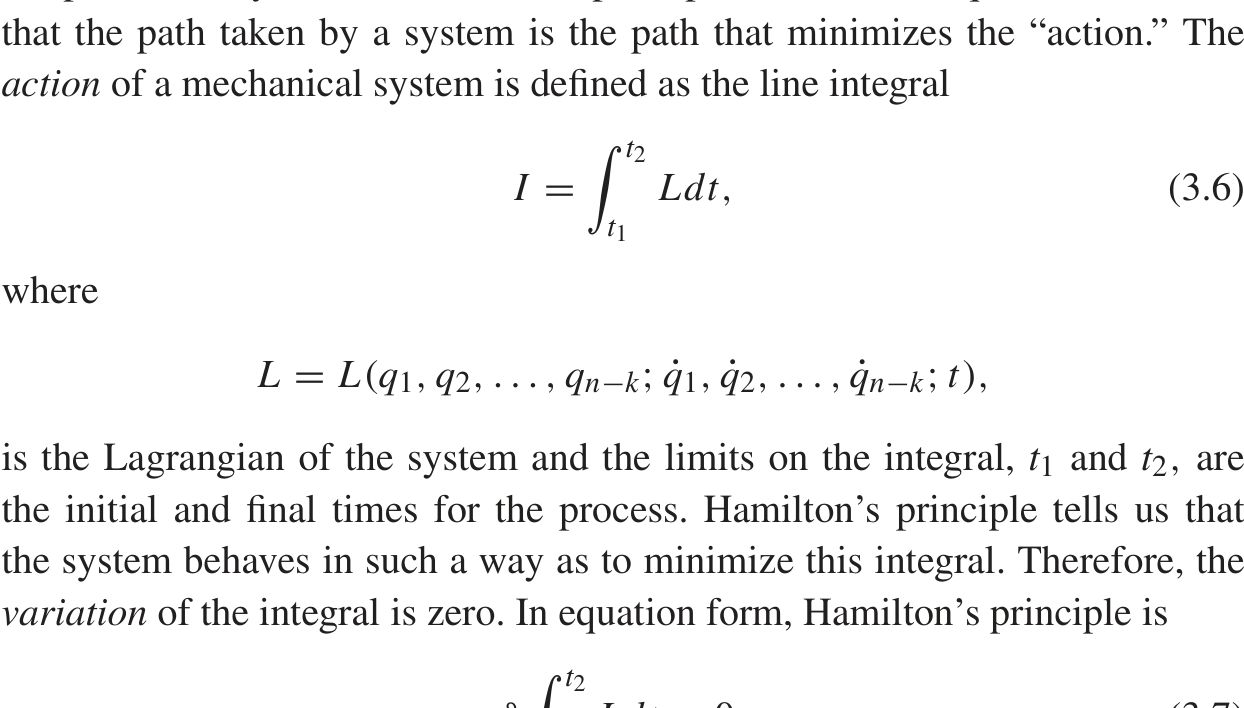
\includegraphics[width=0.55\linewidth]{../Figures/fig_3_1.png}
\caption{图 3.1}
\end{figure}

假定其中一条路径就是使作用量取极小值的路径。（它就是"真实"路径。）那么，沿着该路径，$\delta\int_{t_1}^{t_2}L\,dt = 0$。对于系统实际遵循的路径，积分取极小值，而沿任何其他路径，作用量的值都更大。

\section*{3.3  拉格朗日方程的推导}

我们现在可以从哈密顿原理推导拉格朗日方程，只要认识到把变量从 $(x, y, y')$ 简单改换为 $L(t, q, \dot{q})$，就可以使哈密顿原理几乎平凡地改写为变分法的语言。哈密顿原理告诉我们，力学系统将沿位形空间中由 $q = q(t)$ 给出的一条路径运动，使得积分
\[
\int_{t_i}^{t_f}L(t, q, \dot{q})\,dt
\]
取极小值。（注意，在这里拉格朗日量应视为一个泛函。）

现在，若 $q = q(t)$ 是使积分取极小值的路径，则 $L$ 必须满足欧拉-拉格朗日方程
\[
\frac{d}{dt}\frac{\partial L}{\partial\dot{q}} - \frac{\partial L}{\partial q} = 0.
\tag{3.8}
\]
习惯上把这个方程简称为"拉格朗日"方程。它可以很容易地推广到由任意多个广义坐标描述的系统。

\begin{exercise}
证明方程(3.7)可以导出方程(3.8)。以第 2.2 节给出的论证作为引导。
\end{exercise}

\section*{3.4  推广到多个坐标}

考虑一个由广义坐标 $q_1, q_2, \ldots, q_n$ 描述的系统。我们假定这些坐标都是独立的。该系统的拉格朗日量为 $L(q_1, q_2, \ldots, q_n, \dot{q}_1, \dot{q}_2, \ldots, \dot{q}_n, t)$。我们的计划是证明如下形式的拉格朗日方程
\[
\frac{d}{dt}\frac{\partial L}{\partial\dot{q}_i} - \frac{\partial L}{\partial q_i} = 0,
\qquad i = 1, \ldots, n
\]
由哈密顿原理导出。推导过程与第 2.3 节给出的相似。

回想函数变分的定义。若
\[
f = f(q_i, \dot{q}_i, t),
\]
则
\[
\delta f = \sum_i\left(\frac{\partial f}{\partial q_i}\delta q_i + \frac{\partial f}{\partial\dot{q}_i}\delta\dot{q}_i\right).
\]
注意，在这个表达式中，时间假定不变。

再次考虑方程(3.7)形式的哈密顿原理，即
\[
\delta\int_{t_1}^{t_2}L\,dt = \delta\int_{t_1}^{t_2}L(q_1, q_2, \ldots, q_n, \dot{q}_1, \dot{q}_2, \ldots, \dot{q}_n, t)\,dt = 0,
\]
或
\[
\delta I = 0,
\]
其中作用量用 $I$ 表示，积分沿物理系统实际遵循的"路径"进行。注意，对于该路径，作用量的变分为零。然而，和前面一样，端点之间存在着无限多条可能的路径，我们将它们表示为
\[
Q_i(t) = q_i(t) + \epsilon\eta_i(t).
\]
在这种情况下，作用量可以看作 $\epsilon$ 的函数。拉格朗日量 $L$ 是 $Q_i$、$\dot{Q}_i$ 以及（间接地）$\epsilon$ 的函数。因此，作用量的变分为
\[
\delta I = \int_{t_1}^{t_2}\delta L\,dt = \int_{t_1}^{t_2}\left(\frac{\partial L}{\partial Q_i}\delta Q_i + \frac{\partial L}{\partial\dot{Q}_i}\delta\dot{Q}_i\right)dt.
\]
注意到 $Q_i$ 和 $\dot{Q}_i$ 是 $\epsilon$ 的函数，我们写为
\[
\delta I = \frac{\partial I}{\partial\epsilon}d\epsilon = \int_{t_1}^{t_2}\left(\frac{\partial L}{\partial Q_i}\frac{\partial Q_i}{\partial\epsilon}d\epsilon + \frac{\partial L}{\partial\dot{Q}_i}\frac{\partial\dot{Q}_i}{\partial\epsilon}d\epsilon\right)dt.
\]
第二项可以分部积分。（注意，这里的数学步骤与从方程(2.6)到方程(2.7)的步骤几乎完全相同。）

我们得到
\[
\begin{aligned}
\int_{t_1}^{t_2}\frac{\partial L}{\partial\dot{Q}_i}\frac{\partial\dot{Q}_i}{\partial\epsilon}d\epsilon\,dt
&= \int_{t_1}^{t_2}\frac{\partial L}{\partial\dot{Q}_i}\frac{\partial^2 Q_i}{\partial\epsilon\partial t}\,dt\,d\epsilon
= \int_{t_1}^{t_2}\frac{\partial L}{\partial\dot{Q}_i}\frac{\partial}{\partial\epsilon}\left(\frac{\partial Q_i}{\partial t}\right)dt\,d\epsilon\\
&= \left.\frac{\partial L}{\partial\dot{Q}_i}\frac{\partial Q_i}{\partial\epsilon}\right|_{t_1}^{t_2}
- \int_{t_1}^{t_2}\frac{\partial Q_i}{\partial\epsilon}\frac{d}{dt}\frac{\partial L}{\partial\dot{Q}_i}\,dt\,d\epsilon\\
&= -\int_{t_1}^{t_2}\frac{\partial Q_i}{\partial\epsilon}\frac{d}{dt}\frac{\partial L}{\partial\dot{Q}_i}\,dt\,d\epsilon,
\end{aligned}
\]
其中我们利用了如下事实：因为所有曲线都经过端点，所以
\[
\left.\frac{\partial Q_i}{\partial\epsilon}\right|_{t_1}^{t_2} = 0.
\]
因此，
\[
\begin{aligned}
\delta I &= \int_{t_1}^{t_2}\left(\frac{\partial L}{\partial Q_i}\frac{\partial Q_i}{\partial\epsilon} - \frac{\partial Q_i}{\partial\epsilon}\frac{d}{dt}\frac{\partial L}{\partial\dot{Q}_i}\right)d\epsilon\,dt\\
&= \int_{t_1}^{t_2}\left(\frac{\partial L}{\partial Q_i} - \frac{d}{dt}\frac{\partial L}{\partial\dot{Q}_i}\right)\frac{\partial Q_i}{\partial\epsilon}\,d\epsilon\,dt\\
&= \int_{t_1}^{t_2}\left(\frac{\partial L}{\partial Q_i} - \frac{d}{dt}\frac{\partial L}{\partial\dot{Q}_i}\right)\delta Q_i\,dt.
\end{aligned}
\]
当 $\epsilon = 0$ 时，$\delta I = 0$，因为 $I$ 沿路径 $q_i = q_i(t)$ 取极小值。所以
\[
[\delta I]_{\epsilon=0} = 0 = \int_{t_1}^{t_2}\left(\frac{\partial L}{\partial q_i} - \frac{d}{dt}\frac{\partial L}{\partial\dot{q}_i}\right)\delta q_i\,dt.
\tag{3.9}
\]
由于 $\delta q_i$ 是独立的，这个表达式要等于零，唯一的可能就是把括号中的所有项都取为零。因此，拉格朗日方程得证。

\section*{3.5  约束与拉格朗日 λ 方法}

我们现在应用第 2.4.1 节的拉格朗日 λ 方法来确定作用在系统上的约束力。

设一个系统由 $n$ 个广义坐标 $q_1, q_2, \ldots, q_n$ 描述。进一步假定该系统受到 $k$ 个完整约束，因此有 $k$ 个联系这些坐标的方程。显然，并非所有广义坐标都是独立的，所以我们本可以用这 $k$ 个约束方程把广义坐标的数目减少到 $n - k$。然而，目前我们宁愿使用全部 $n$ 个坐标。

系统的行为由哈密顿原理描述，
\[
\delta I = \delta\int_{t_1}^{t_2}L\,dt = 0,
\]
以及 $k$ 个约束方程
\[
f_j(q_1, q_2, \ldots, q_n) = 0,
\qquad j = 1, \ldots, k.
\tag{3.10}
\]
如果所有坐标都是独立的，哈密顿原理将导出 $n$ 个如下形式的方程
\[
\frac{d}{dt}\frac{\partial L}{\partial\dot{q}_i} - \frac{\partial L}{\partial q_i} = 0,
\qquad i = 1, \ldots, n.
\tag{3.11}
\]
但（现在）我们还不能这样写，因为正如方程(3.9)后面所指出的，这一结果依赖于所有 $\delta q$ 都是独立的。

方程(3.10)表示完整约束。因此
\[
\delta f_j = \frac{\partial f_j}{\partial q_1}\delta q_1 + \frac{\partial f_j}{\partial q_2}\delta q_2 + \cdots + \frac{\partial f_j}{\partial q_n}\delta q_n = 0.
\]
也就是说，
\[
\sum_{i=1}^{n}\frac{\partial f_j}{\partial q_i}\delta q_i = 0,
\qquad j = 1, \ldots, k.
\tag{3.12}
\]
这里的系数 $\partial f_j/\partial q_i$ 是 $q_i$ 的函数。如果方程(3.12)成立，那么把它乘以某个量（称之为 $\lambda_j$）不会产生任何影响，所以我们可以把它写成
\[
\lambda_j\sum_{i=1}^{n}\frac{\partial f_j}{\partial q_i}\delta q_i = 0.
\]
这些 $\lambda$ 是未定乘子。共有 $k$ 个这样的方程，把它们相加仍然为零，所以
\[
\sum_{j=1}^{k}\lambda_j\sum_{i=1}^{n}\frac{\partial f_j}{\partial q_i}\delta q_i = 0.
\]
再者，我们可以从 $t_i$ 积分到 $t_f$，仍然不会改变其值为零这一事实。这给出有用的关系
\[
\int_{t_1}^{t_2}dt\left(\sum_{j=1}^{k}\lambda_j\sum_{i=1}^{n}\frac{\partial f_j}{\partial q_i}\delta q_i\right) = 0.
\tag{3.13}
\]

方程(3.9)可以写成
\[
\int_{t_1}^{t_2}dt\left(\frac{\partial L}{\partial q_i} - \frac{d}{dt}\frac{\partial L}{\partial\dot{q}_i}\right)\delta q_i = 0.
\tag{3.14}
\]
将方程(3.13)和(3.14)相加，我们得到
\[
\int_{t_1}^{t_2}dt\left(\frac{\partial L}{\partial q_i} - \frac{d}{dt}\frac{\partial L}{\partial\dot{q}_i} + \sum_{j=1}^{k}\lambda_j\frac{\partial f_j}{\partial q_i}\right)\delta q_i = 0.
\tag{3.15}
\]
并非所有 $\delta q$ 都是独立的；它们由 $k$ 个约束方程联系起来。然而，其中有 $n - k$ 个是独立的，对于这些坐标，方程(3.15)中括号内的项必须为零。对于其余 $k$ 个方程，我们可以选择未定乘子 $\lambda_j$，使得
\[
\frac{\partial L}{\partial q_i} - \frac{d}{dt}\frac{\partial L}{\partial\dot{q}_i} + \sum_{j=1}^{k}\lambda_j\frac{\partial f_j}{\partial q_i} = 0.
\]
因此，对所有 $q_i$，我们都有如下关系
\[
\frac{d}{dt}\frac{\partial L}{\partial\dot{q}_i} - \frac{\partial L}{\partial q_i} = \sum_{j=1}^{k}\lambda_j\frac{\partial f_j}{\partial q_i},
\qquad i = 1, \ldots, n.
\tag{3.16}
\]
方程(3.16)是 $n$ 个方程，方程(3.10)给出 $k$ 个方程，所以我们有 $n + k$ 个方程，可以解出 $q$ 和 $\lambda$ 的表达式。

我们现在来说明 $\lambda$ 如何与约束的广义力联系起来。考虑写成尼尔森形式（方程(3.4)）的拉格朗日方程。我们把该方程写成如下方式，在其中把可由势函数 $V$ 导出的保守力 $Q_i^c$ 与约束力 $Q_i^{nc}$ 分离开来（约束力一般来说不能由只依赖于坐标的势导出）：
\[
\frac{d}{dt}\frac{\partial T}{\partial\dot{q}_i} - \frac{\partial T}{\partial q_i} = Q_i^c + Q_i^{nc}.
\]
保守力 $Q^c$ 可以表示为 $-\partial V/\partial q_i$。假定 $\partial V/\partial\dot{q}_i = 0$，我们可以把这个方程写成
\[
\frac{d}{dt}\frac{\partial L}{\partial\dot{q}_i} - \frac{\partial L}{\partial q_i} = Q_i^{nc}.
\tag{3.17}
\]

但方程(3.16)和(3.17)必然完全相同。因此我们得到如下表达式
\[
Q_i^{nc} = \sum_{j=1}^{k}\lambda_j\frac{\partial f_j}{\partial q_i},
\]
于是我们得到了所要求的约束力表达式。

\begin{example}
考虑一个半径为 $R$ 的圆盘沿长为 $l$、倾角为 $\alpha$ 的斜面滚下。求运动方程、角加速度以及使圆盘无滑动滚动所需的约束力。
\begin{figure}[h]
\centering
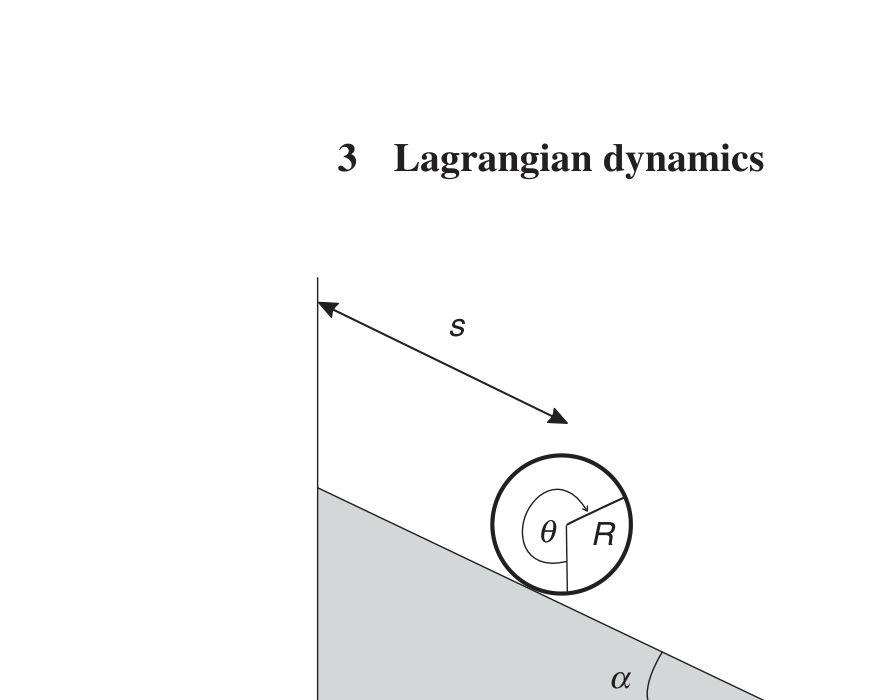
\includegraphics[width=0.55\linewidth]{../Figures/fig_3_2.png}
\caption{图 3.2}
\end{figure}

解 3.1 圆盘的转动惯量为 $I = \frac{1}{2}MR^2$，动能为 $T = \frac{1}{2}M\dot{s}^2 + \frac{1}{2}I\dot{\theta}^2$。势能为 $V = Mg(l - s)\sin\alpha$。因此，
\[
L = \frac{1}{2}M\dot{s}^2 + \frac{1}{4}MR^2\dot{\theta}^2 + Mg(s - l)\sin\alpha.
\]
圆盘受到无滑动滚动的约束。因此，
\[
f(s, \theta) = s - R\theta = 0.
\]
这是一个完整约束。因此，
\[
\frac{d}{dt}\frac{\partial L}{\partial\dot{s}} - \frac{\partial L}{\partial s} = \lambda\frac{\partial f}{\partial s},
\]
其中 $\partial f/\partial s = 1$，
\[
\frac{d}{dt}\frac{\partial L}{\partial\dot{\theta}} - \frac{\partial L}{\partial\theta} = \lambda\frac{\partial f}{\partial\theta},
\]
其中 $\partial f/\partial\theta = -R$。

进行所示运算，我们得到两个运动方程
\[
\frac{d}{dt}\left(M\dot{s}\right) - Mg\sin\alpha = \lambda,
\]
\[
\frac{d}{dt}\left(\frac{1}{2}MR^2\dot{\theta}\right) = -R\lambda.
\]
此外，由约束方程我们得到另一个方程，即
\[
\ddot{\theta} = \ddot{s}/R.
\]
你可以很容易地证明
\[
\ddot{\theta} = \frac{2g\sin\alpha}{3R},
\]
以及
\[
\ddot{s} = \frac{2}{3}g\sin\alpha.
\]
由此得到
\[
\lambda = M\ddot{s} - Mg\sin\alpha = -\frac{1}{3}Mg\sin\alpha.
\]
现在约束力由下式给出
\[
Q_s = \lambda\frac{\partial f}{\partial s} = -\frac{1}{3}Mg\sin\alpha = \text{法向力},
\]
以及
\[
Q_\theta = \lambda\frac{\partial f}{\partial\theta} = \frac{1}{3}MgR\sin\alpha = \text{力矩}.
\]
$Q_s$ 和 $Q_\theta$ 是使圆盘无滑动地滚下平面所需的广义力。
\end{example}

\begin{exercise}
补全上面例子中被省略的步骤，证明 $\ddot{\theta} = (2/3)g\sin\alpha/R$ 和 $\ddot{s} = (2/3)g\sin\alpha$。
\end{exercise}

\section*{3.6  非完整约束}

某些非完整约束也可以用拉格朗日 λ 方法处理，如第 2.4.2 节所述。假定非完整约束可以表示为坐标微分之间的关系。例如，如果只有一个这样的约束，它由下式给出
\[
A_1dq_1 + A_2dq_2 + \cdots + A_ndq_n = 0,
\]
其中 $A$ 是 $q$ 的已知函数。如果这个关系对 $dq$ 成立，那么它对 $\delta q$ 也成立，所以我们可以写
\[
A_1\delta q_1 + A_2\delta q_2 + \cdots + A_n\delta q_n = 0.
\tag{3.18}
\]
但最后这个表达式与完整约束的 $\delta f$ 表达式具有相同的形式，我们把它写为
\[
\delta f = \frac{\partial f}{\partial q_1}\delta q_1 + \frac{\partial f}{\partial q_2}\delta q_2 + \cdots + \frac{\partial f}{\partial q_n}\delta q_n = 0.
\]
因此，我们可以使用与之前完全相同的推理，只需把 $\partial f/\partial q$ 换成 $A$。（不过要注意，虽然 $A$ 是已知量，但它们并不是某个已知函数的偏导数。）因此，如果我们唯一的非完整约束可以表示为方程(3.18)的形式，那么拉格朗日方程为
\[
\frac{d}{dt}\frac{\partial L}{\partial\dot{q}_i} - \frac{\partial L}{\partial q_i} = \lambda A_i,
\qquad i = 1, 2, \ldots, n.
\]
如果非完整约束不止一个，我们就需要推广这一关系。例如，如果有 $m$ 个非完整约束，我们将有 $i$ 个如下形式的方程
\[
\frac{d}{dt}\frac{\partial L}{\partial\dot{q}_i} - \frac{\partial L}{\partial q_i} = \sum_{k=1}^{m}\lambda_kA_{ki},
\qquad i = 1, 2, \ldots, n.
\]
我们甚至可以把这一方法用于具有如下形式的含时（"rheonomic"）约束：
\[
\sum_{i=1}^{n}A_{ki}dq_i + B_kdt = 0,
\qquad k = 1, 2, \ldots, m.
\]
这里的系数（$A$ 和 $B$）一般来说是坐标和时间的函数。和前面一样，我们可以用 $\delta$ 替换 $d$，并把这些约束写成如下形式
\[
\sum_{i=1}^{n}A_{ki}\delta q_i + B_k\delta t = 0,
\qquad k = 1, 2, \ldots, m.
\]

$\delta t$ 的系数（即 $B$）不进入运动方程，因为在虚位移 $\delta q_i$ 期间时间是冻结的。因此运动方程取熟悉的形式
\[
\frac{d}{dt}\frac{\partial L}{\partial\dot{q}_i} - \frac{\partial L}{\partial q_i} = \sum_{k=1}^{m}\lambda_kA_{ki},
\qquad i = 1, 2, \ldots, n.
\]
不过要注意，$B$ 会进入速度之间的关系，于是
\[
A_{i1}\dot{q}_1 + A_{i2}\dot{q}_2 + \cdots + A_{in}\dot{q}_n + B_i = 0,
\qquad i = 1, 2, \ldots, n.
\]

\section*{3.7  虚功}

我们现在要比第 1.6 节更详细地考察虚功的概念。一个力学系统处于平衡，当且仅当所有"外加"力的总虚功为零。（外加力是施加在系统上的力，不包括约束力。\footnote{约束力常常被称为"反作用"力。}）系统处于平衡时的虚功原理用数学表示为
\[
\delta W = \sum_j Q_j\delta q_j = 0.
\]
这里的虚位移 $\delta q_i$ 满足所有约束。注意，虚功原理是一个变分原理。

把虚功原理与牛顿力学中的平衡概念加以对照是很有趣的。在牛顿力学中，当系统处于平衡时，作用在它上面的所有力的矢量和为零。也就是说，牛顿力学用力来取代约束。另一方面，分析力学则不考虑反作用力，只考虑外加力；然而，它要求任何虚位移都必须满足系统的约束。（正如我们将看到的，考虑违反约束的虚位移使我们能够确定约束力。）

用矢量记号，广义力就是实际力的分量，虚功原理可以表示为
\[
\mathbf{F}_1\cdot\delta\mathbf{r}_1 + \mathbf{F}_2\cdot\delta\mathbf{r}_2 + \cdots + \mathbf{F}_N\cdot\delta\mathbf{r}_N = 0.
\]
用笛卡尔坐标表示，这就是
\[
F_{1x}\delta x_1 + F_{1y}\delta y_1 + \cdots + F_{Nz}\delta z_N = 0.
\]

写成这种形式后，我们认识到力与虚位移的标量积都为零。这意味着力 $\mathbf{F}_i$ 垂直于质点 $i$ 的任何允许位移。对于自由质点，所有位移都是允许的，所以合力必须为零。对于被限制在桌面上的质点，力必须垂直于桌面。

如果平衡问题涉及约束，那么平衡条件可以用拉格朗日 λ 方法来确定。

我们已经论证了虚功原理，但还没有证明它。让我们把它作为一条公设。（事实上，它是分析力学唯一的公设，并且既适用于动力学情形，也适用于平衡情形。\footnote{关于该公设的讨论，见 Lanczos，前引书，第 76 页。}）

\textbf{公设} 系统处于平衡时虚功为零，
\[
\delta W = 0.
\]
由于牛顿动力学指出，处于平衡的系统上所受的总力为零，我们得出结论：反作用力与外加力大小相等、方向相反。因此，这条公设可以用反作用力表述如下。

\textbf{公设} 对于满足系统约束的任何虚位移，任何反作用力的虚功为零。

\begin{exercise}
假设外加力可由一个标量函数导出。证明平衡状态由势能的驻值给出，即 $\delta V = 0$。
\end{exercise}

\subsection*{3.7.1  拉格朗日乘子的物理意义}

处于平衡时，外加力的虚功为零：
\[
\delta W = 0.
\]
如果外加力可以由一个势能导出（$F_i = -\partial V/\partial q_i$），那么虚功就等于势能变分的负值，因为
\[
\delta W = \sum_i F_i\delta q_i = -\sum_i(\partial V/\partial q_i)\delta q_i = -\delta V.
\]
如果物理系统受到如下给出的完整约束
\[
f(q_1, \ldots, q_n) = 0,
\]
那么拉格朗日 λ 方法要求
\[
\delta(L + \lambda f) = 0.
\]
（参见方程(2.24)。）由于 $\lambda$ 未确定，我们完全可以用 $-\lambda$，并定义修正的拉格朗日量
\[
L' = L - \lambda f.
\]
由于 $L = T - V$，这等价于定义一个修正的势能 $V + \lambda f$。因此，$\delta W = 0$ 等价于
\[
\delta(V + \lambda f) = 0.
\]
如果我们允许广义坐标有任意变分（而不只是那些满足约束的变分），那么反作用力就会作用在系统上。因此，$\lambda f$ 这一项可以解释为与约束力相关的势能。于是，反作用力的第 $\xi$ 个分量为
\[
F_i = -\frac{\partial(\lambda f)}{\partial\xi_i} = -\lambda\frac{\partial f}{\partial\xi_i} - \frac{\partial\lambda}{\partial\xi_i}f.
\]
但 $f = 0$，所以
\[
F_i = -\lambda\frac{\partial f}{\partial\xi_i}.
\]
我们得出结论：完整约束由可由一个标量函数导出的力来维持。

正如我们所看到的，某些非完整约束也可以用拉格朗日 λ 方法处理；然而，这些力（摩擦就是一个例子）不能由标量函数导出。

\begin{example}
你可能已经用微积分（也许是在以前的力学课程中）证明过，由悬挂的链条或重绳形成的曲线是一条悬链线。这个问题也可以用变分技术来求解。要极小化的量是势能 $V = V(y)$。问题是要在链条长度为一给定常数的约束下确定 $y = y(x)$。用变分的语言来说，我们希望在给定 $\delta V = 0$ 且受到如下约束的条件下确定 $y = y(x)$：
\[
\int_{x_1}^{x_2}ds = \text{常数} = \text{长度} = l.
\]
解 3.2 这个约束可以表示为
\[
l = \int_{x_1}^{x_2}\sqrt{1 + y'^2}\,dx.
\]
一段长度为 $ds$ 的链条的势能为 $dV = (dm)gh = \rho gy\,ds$。略去不必要的常数，
\[
V = \int_{x_1}^{x_2}y\,ds = \int_{x_1}^{x_2}y\sqrt{1 + y'^2}\,dx.
\]
拉格朗日 λ 方法给出
\[
\delta\int_{x_1}^{x_2}(y + \lambda)\sqrt{1 + y'^2}\,dx = 0.
\]
确定该曲线的方程留作练习。
\end{example}

\begin{exercise}
前面例子中的泛函不显含 $x$。按照第 2.2.2 节中讨论的方式重新表述该问题，并证明该曲线是一条悬链线。
\end{exercise}

\begin{exercise}
考虑一个由质量 $m$ 组成、被长度为 $l$ 的细线约束在圆弧上摆动的单摆。假设 $r$ 和 $\theta$ 都是变量。写出拉格朗日方程，并利用 λ 方法确定细线中的张力。用初等方法进行核对。
\end{exercise}

\section*{3.8  拉格朗日方程的不变性}

拉格朗日方程在点变换下不变。点变换是把一组坐标 $q_1, q_2, \ldots, q_n$ 变换到一组坐标 $s_1, s_2, \ldots, s_n$ 的变换，使得"q 空间"中的每一个点 $P_q$ 都对应着"s 空间"中的一个点 $P_s$。变换方程具有如下形式
\[
\begin{aligned}
q_1 &= q_1(s_1, s_2, \ldots, s_n, t),\\
&\vdots\\
q_n &= q_n(s_1, s_2, \ldots, s_n, t).
\end{aligned}
\]
不难证明拉格朗日方程在点变换下不变。（也就是说，它们保持相同的形式。参见本章末尾的问题 3.3。）然而，要理解这种不变性的意义可能更难一些，所以让我们更详细地考察它。
\begin{figure}[h]
\centering
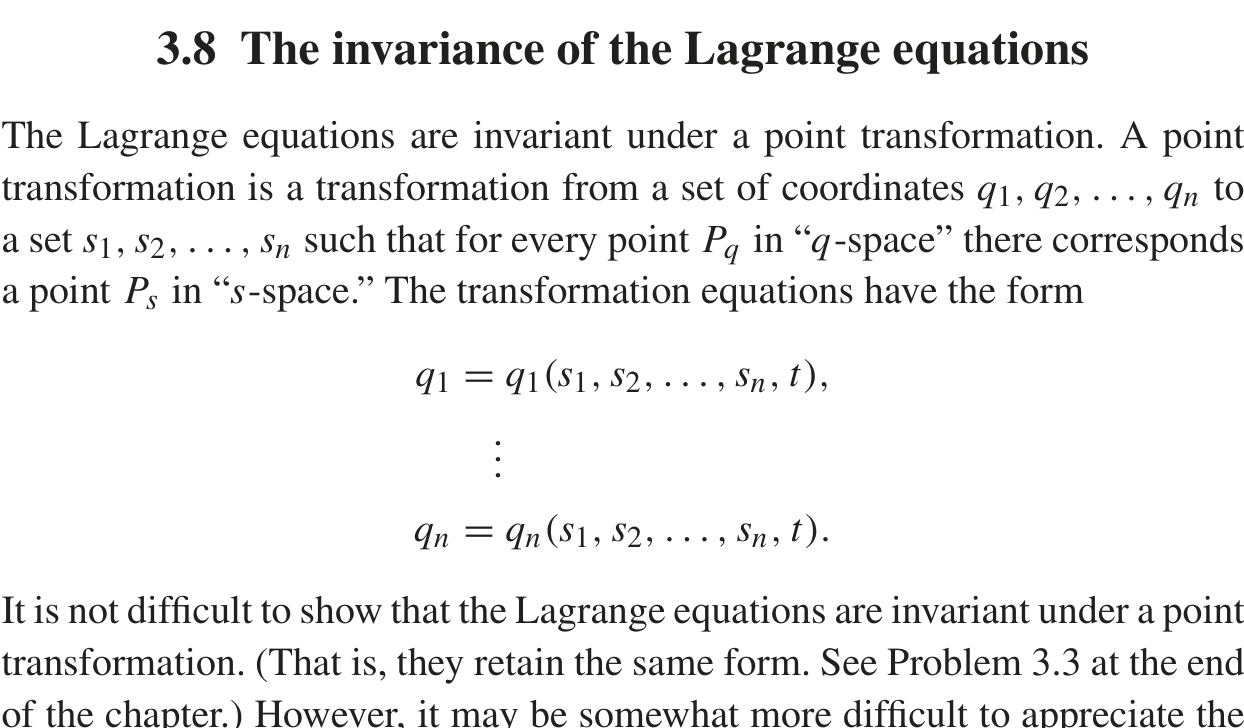
\includegraphics[width=0.55\linewidth]{../Figures/fig_3_3.png}
\caption{图 3.3}
\end{figure}

系统由单个点表示。随时间推移，这个点沿一条曲线运动。\footnote{我们可以把时间作为另一个坐标，并在 $(n + 1)$ 维位形空间中用点表示系统。在这个空间中，系统描出一条给出系统历史的曲线或"世界线"。}系统沿使作用量取极小值的曲线 $C$ 从端点 $A$ 运动到端点 $B$。通过考虑同一端点之间的变分路径，并要求"真实"路径的作用量积分为驻值，我们得到条件
\[
\frac{d}{dt}\frac{\partial L}{\partial\dot{q}_i} - \frac{\partial L}{\partial q_i} = 0,
\qquad i = 1, \ldots, n.
\]
设坐标 $q_i$ 通过点变换变换为 $s_i$。端点变换为 $\tilde{A}$、$\tilde{B}$，曲线 $C$ 变换为 $\tilde{C}$，如图所示。
\begin{figure}[h]
\centering
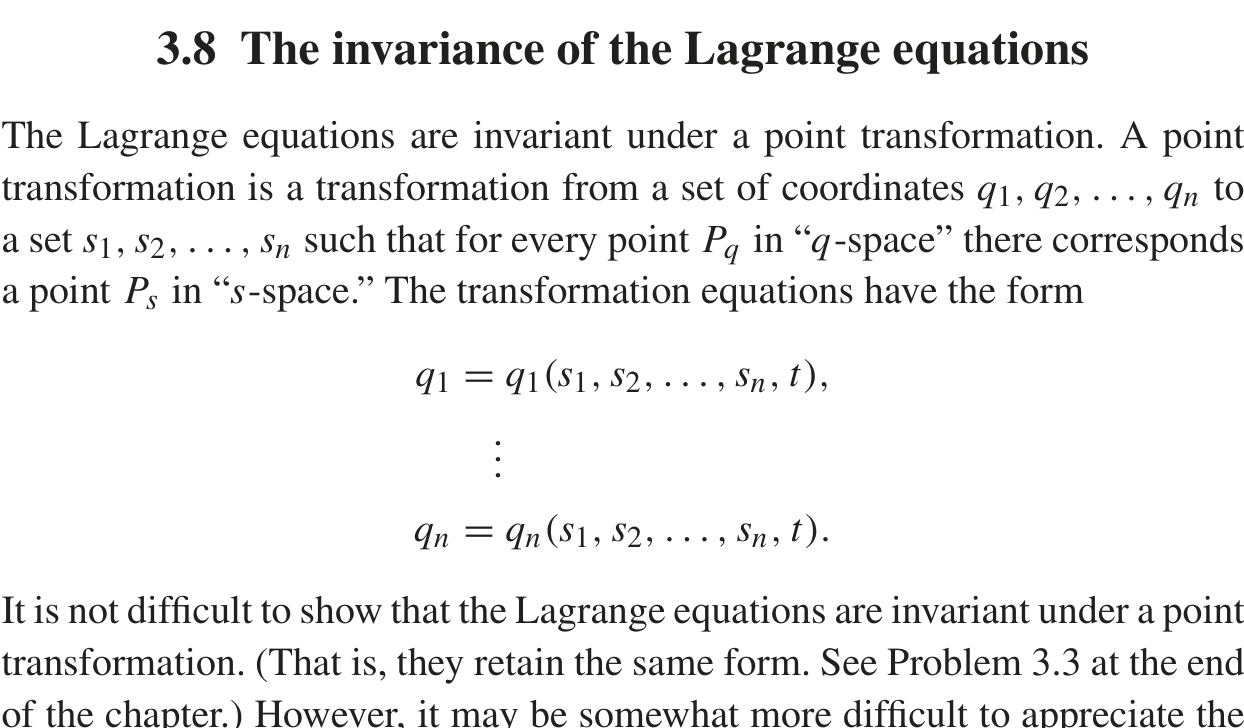
\includegraphics[width=0.55\linewidth]{../Figures/fig_3_3.png}
\caption{图 3.3}
\end{figure}

在任何坐标系中，端点之间的"真实"路径都使作用量积分取极小值，因此拉格朗日方程在新坐标系中成立。不过要注意，尽管 $L$ 的值在两个坐标系中相同，其形式却可能大不相同。拉格朗日方程的不变性使我们能够选择任何一组使方程最容易求解的坐标。（不变性原理在狭义相对论理论中成为一个公设，爱因斯坦在那里假定物理定律在惯性参考系之间的变换下不变。）

某个特定 $i$ 的拉格朗日运动方程在两个系统中一般来说并不相同，但完整的方程组是等价的。出于这个原因，实际上应把这些方程称为协变的，而不是不变的。例如，若
\[
L = \frac{1}{2}\dot{x}^2 + \frac{1}{2}\dot{y}^2 + (x^2 + y^2)^{-1/2},
\]
点变换 $x = r\cos\theta$，$y = r\sin\theta$ 给出拉格朗日量
\[
L = \frac{1}{2}\dot{r}^2 + \frac{1}{2}r^2\dot{\theta}^2 + \frac{1}{r}.
\]
用 $x$ 和 $y$ 表示的运动方程为
\[
\ddot{x} = -\frac{x}{(x^2 + y^2)^{3/2}},
\qquad \ddot{y} = -\frac{y}{(x^2 + y^2)^{3/2}},
\]
而用 $r$ 和 $\theta$ 表示的运动方程为
\[
\ddot{r} - r\dot{\theta}^2 + \frac{1}{r^2} = 0,
\qquad \frac{d}{dt}\left(r^2\dot{\theta}\right) = 0.
\]
尽管这些运动方程在形式上大不相同，它们却给出相同的结果，并且对于一组特定的位置和速度参数，它们给出的拉格朗日量数值相同。

\section*{3.9  习题}

3.1 假设广义力可由一个与广义速度无关的势导出。证明方程(3.1)可由方程(3.4)导出。
3.2 利用达朗贝尔原理确定下面系统的平衡条件。
\begin{figure}[h]
\centering
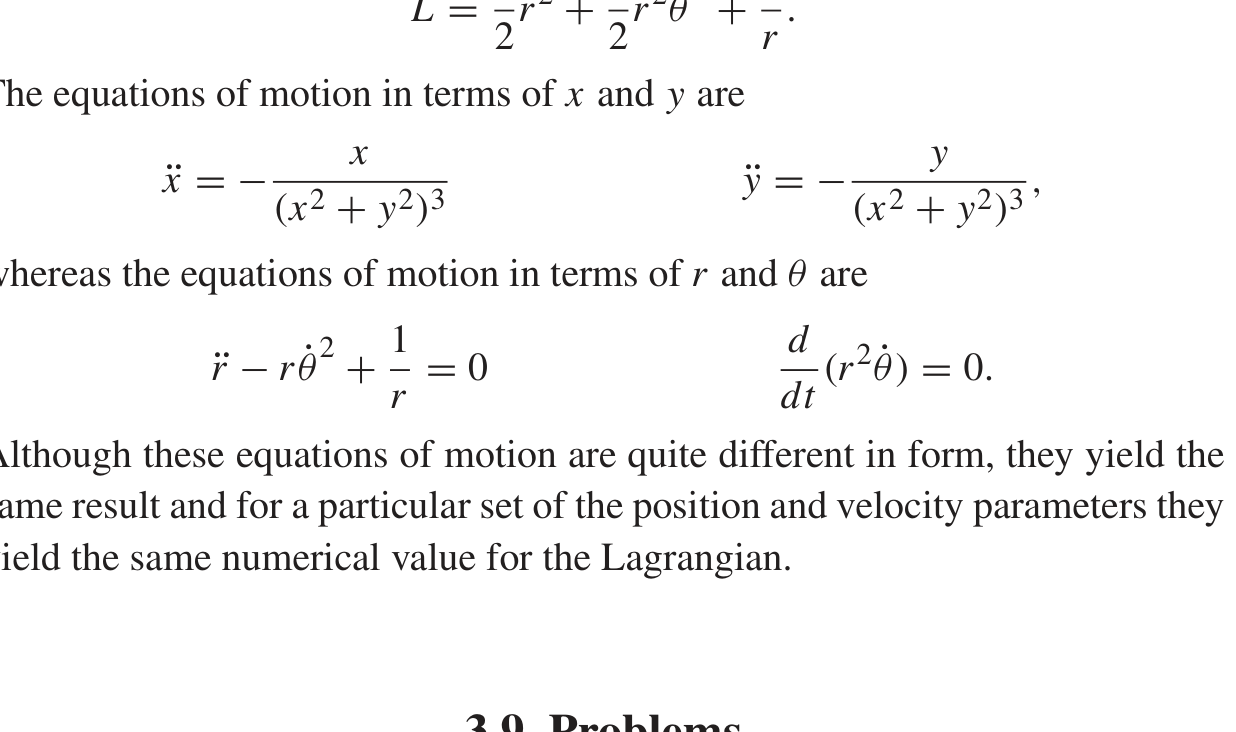
\includegraphics[width=0.55\linewidth]{../Figures/fig_3_4.png}
\caption{图 3.4}
\end{figure}

3.3 若把拉格朗日量用某一组广义坐标 $q_i$ 表示，则拉格朗日运动方程具有如下形式
\[
\frac{d}{dt}\frac{\partial L}{\partial\dot{q}_i} - \frac{\partial L}{\partial q_i} = 0.
\]
假设我们通过所谓的"点变换"从坐标 $q_i$ 变换到一组新坐标 $s_i$：
\[
q_i = q_i(s_1, s_2, \ldots, s_n, t).
\]
证明拉格朗日方程不变。（即证明拉格朗日方程在点变换下不变。）
3.4 考虑一个在恒定引力场中向上抛出的物体。用数值方法证明真实路径的 $\int_{t_1}^{t_2}(T - V)\,dt$ 比任何"假"路径的都小。你可以任选一条"假"路径。
3.5 一条绳索绕过两个无摩擦的木桩，木桩距地面高度为 $h$，水平间隔为 $d$。绳索的两端位于地面上。确定绳索悬垂部分的曲线方程。
3.6 一个质点在一个倒置半球的外表面上滑动。利用拉格朗日乘子，确定作用在该质点上的反作用力。质点在何处离开半球面？
3.7 一个质量为 $M$、倾角为 $\theta$ 的直角三角形楔块可以在无摩擦的水平面上滑动。一个质量为 $m$ 的物块放在楔块上，它也可以在楔块的无摩擦斜面上滑动。用拉格朗日乘子方法确定楔块和物块的运动方程。确定约束力。
3.8 一个质量为 $m_1$ 的质点通过一根不可伸长、无质量的细绳与质量为 $m_2$ 的质点相连。质点 $m_1$ 可以在无摩擦的桌面上自由滑动。细绳穿过桌面上的一个小孔，$m_2$ 在桌面下方自由悬挂，并且只允许沿竖直方向运动。只有当 $m_1$ 沿绕过孔穴的路径运动时，这一装置才是稳定的。写出该系统的拉格朗日量。求解运动方程。
3.9 一个自由刚体可以绕任意轴转动。也就是说，角速度可以有任意方向。考虑刚体中第 $k$ 个点的一个允许位移：
\[
\delta\mathbf{r}_k = \epsilon\times\mathbf{r}_k.
\]
利用虚功原理，证明这蕴含总角动量守恒。
3.10 根据量子力学，一个质量为 $m$ 的质点在边长分别为 $a$、$b$、$c$ 的长方体盒子中的能量为
\[
E = \frac{h^2}{8m}\left(\frac{1}{a^2} + \frac{1}{b^2} + \frac{1}{c^2}\right).
\]
假设盒子的体积恒定，证明当盒子为立方体（$a = b = c$）时能量最小。
3.11 考虑一根长度固定、悬挂在两个固定点之间的缆绳。证明使势能最小的形状是一条双曲余弦曲线。
